\documentclass{unswmaths}
\usepackage{unswshortcuts}
\usepackage{hyperref}
\usepackage{ dsfont }
\usepackage{fullpage}
\begin{document}
\author{Adam J. Gray}
\title{Assignment 3}
\subject{Ergodic Theory}
\studentno{3329798}

\unswtitle

\section{}
    We consider the map
    \begin{align}
        T(x) = 
        \begin{cases}
            2x + \frac{1}{2} & 0 \leq x < \frac{1}{4} \\
            -x + \frac{5}{4} & \frac{1}{4} \leq x < \frac{1}{2} \\
            -2x + \frac{7}{4} & \frac{1}{2} \leq x < \frac{3}{4} \\
            -x + 1 & \frac{3}{4} \leq x \leq 1.
        \end{cases}
    \end{align}
    This has the following plot:
    
    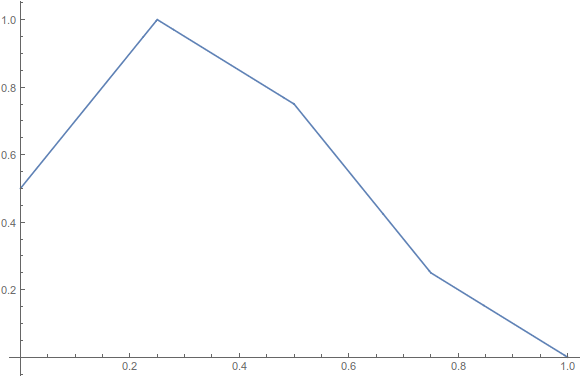
\includegraphics[scale=0.5]{qn_1_map}
\subsection{}
    We have that in general
    \begin{align}
        \mathcal{P}_T f(x) = \sum_{z \in T^{-1} x} \frac{f(z)}{|T'(z)|}.
    \end{align}
    Then in general we have
    \begin{align}
        T'(x) = 
        \begin{cases}
            2 & 0 \leq x < \frac{1}{4} \\
            -1 & \frac{1}{4} \leq x < \frac{1}{2} \\
            -2 & \frac{1}{2} \leq x < \frac{3}{4} \\
            -1 & \frac{3}{4} \leq x \leq 1.
        \end{cases}    
    \end{align}
    Also we can also see that
    \begin{align}
        T^{-1}\{x\} =
        \begin{cases}
            \{1-x\} & 0 \leq x < \frac{1}{4} \\
            \{\frac{7}{8} - \frac{x}{2} \} & \frac{1}{4} \leq x < \frac{1}{2} \\
            \{\frac{7}{8} - \frac{x}{2} \} \cup \{\frac{x}{2} - \frac{1}{4}\} & \frac{1}{2} \leq x < \frac{3}{4} \\
            \{\frac{5}{4} - x\} \cup \{ \frac{x}{2} - \frac{1}{4} \} & \frac{3}{4} \leq x < 1
        \end{cases}
    \end{align}
    thus for $ f_i(x) = \mathds{1}_{I_i}(x) $
    we have that
    \begin{align}
        \mathcal{P}_T f_1(x) &= \frac{1}{2}\mathds{1}_{I_3 \cup I_4}(x) = \frac{1}{2}\mathds{1}_{I_3}(x) + \frac{1}{2}\mathds{1}_{I_4}(x)\\
        \mathcal{P}_T f_2(x) &= \mathds{1}_{I_4}(x) \\
        \mathcal{P}_T f_3(x) &= \frac{1}{2}\mathds{1}_{I_2 \cup I_3}(x) = \frac{1}{2}\mathds{1}_{I_2}(x) + \frac{1}{2}\mathds{1}_{I_3}(x)\\
        \mathcal{P}_T f_4(x) &= \mathds{1}_{I_1}(x)
    \end{align}
\subsection{}
    Let $ \mathcal{S} = \operatorname{span} \bigcup_{i=1}^4 \mathds{1}_{I_i}$.
    
    Let $ f \in \mathcal{S} $ then $ f = \sum_{i=1}^4 \lambda_4 \mathds{1}_{I_i} $ and so by linearity of the Perron-Frobenius operator, we have that $ \mathcal{P}_T(f) = \sum_{i=1}^4 \lambda_4 \mathcal{P}_T(\mathds{1}_{I_i}) $ but from the result above we see that $ \mathcal{P}_T(\mathds{1}_{I_i}) \in \mathcal{S} $ for each $ i $ and so $ \mathcal{P} $ preserves $ \mathcal{S} $
\subsection{}
    We do this by just pluging the basis of $ \mathcal{S} $ into the $ \mathcal{P}_T $ and putting the results in each row of the matrix. Seeing as we already have first part we can just write down the matrix $ M $ as
    \begin{align}
        M = \left[ 
        \begin{array}{cccc}
            0 & 0 & \frac{1}{2} & \frac{1}{2} \\
            0 & 0 & 0 & 1 \\
            0 & \frac{1}{2} & \frac{1}{2} & 0 \\
            1 & 0 & 0 & 0 
        \end{array}
        \right]
    \end{align}
\subsection{}
    Using Mathematica we can calculate the left eigenvector corresponding to eigenvalue 1 which is
    \begin{align}
        \mathbf{v} = (1,\frac{1}{2},1,1)
    \end{align}
    which corresponds to the ACIM (after rescaling)
    \begin{align}
        \frac{8}{7}\left( \mathds{1}_{I_1} + \frac{1}{2}\mathds{1}_{I_2} + \mathds{1}_{I_3} + \mathds{1}_{I_4} \right)
    \end{align}
\clearpage
\section{}
\subsection{}
The following plots we produced by code in \emph{Question\_2\_a.m} available at \url{https://github.com/adamjoshuagray/Honours_Ergodic_Theory/tree/master/Assignment_3}.

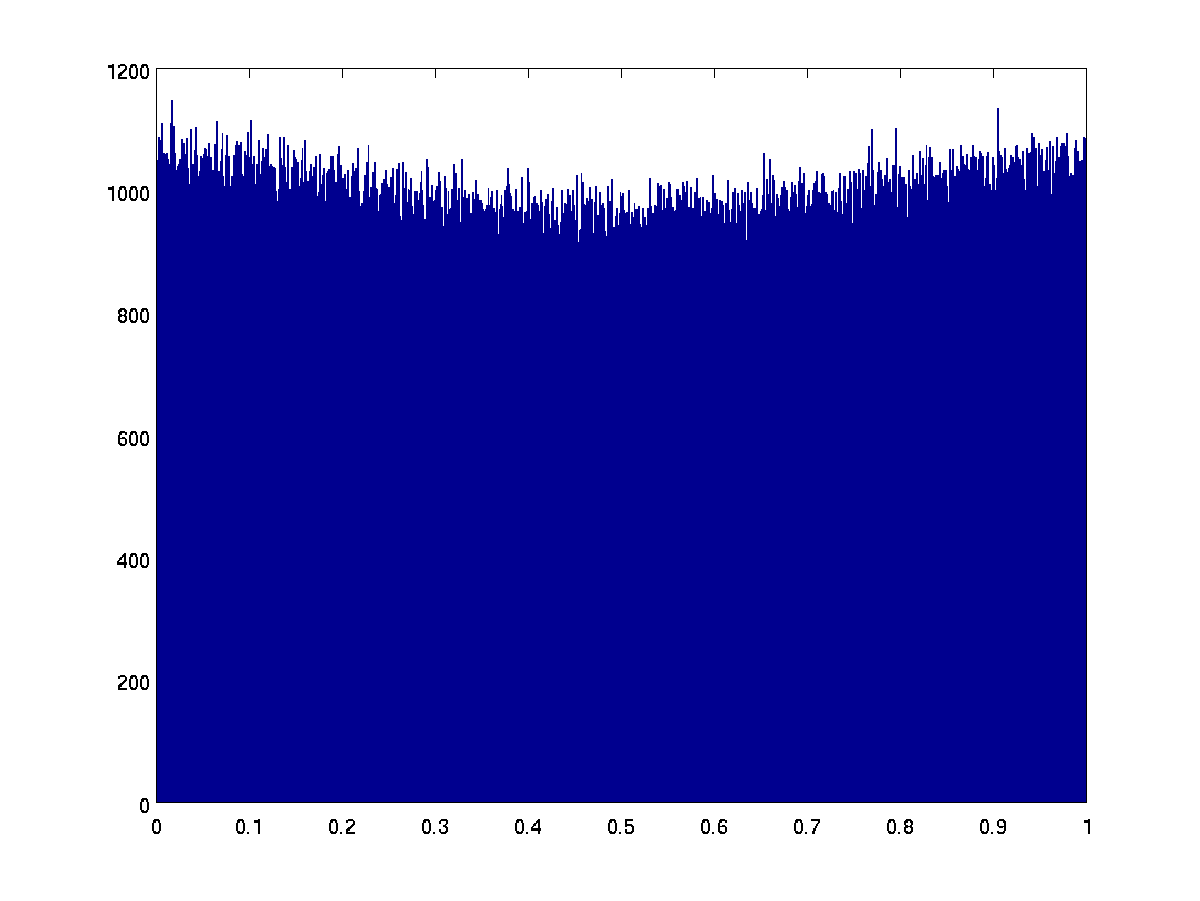
\includegraphics[scale=0.3]{qn_2_a_hist_1}
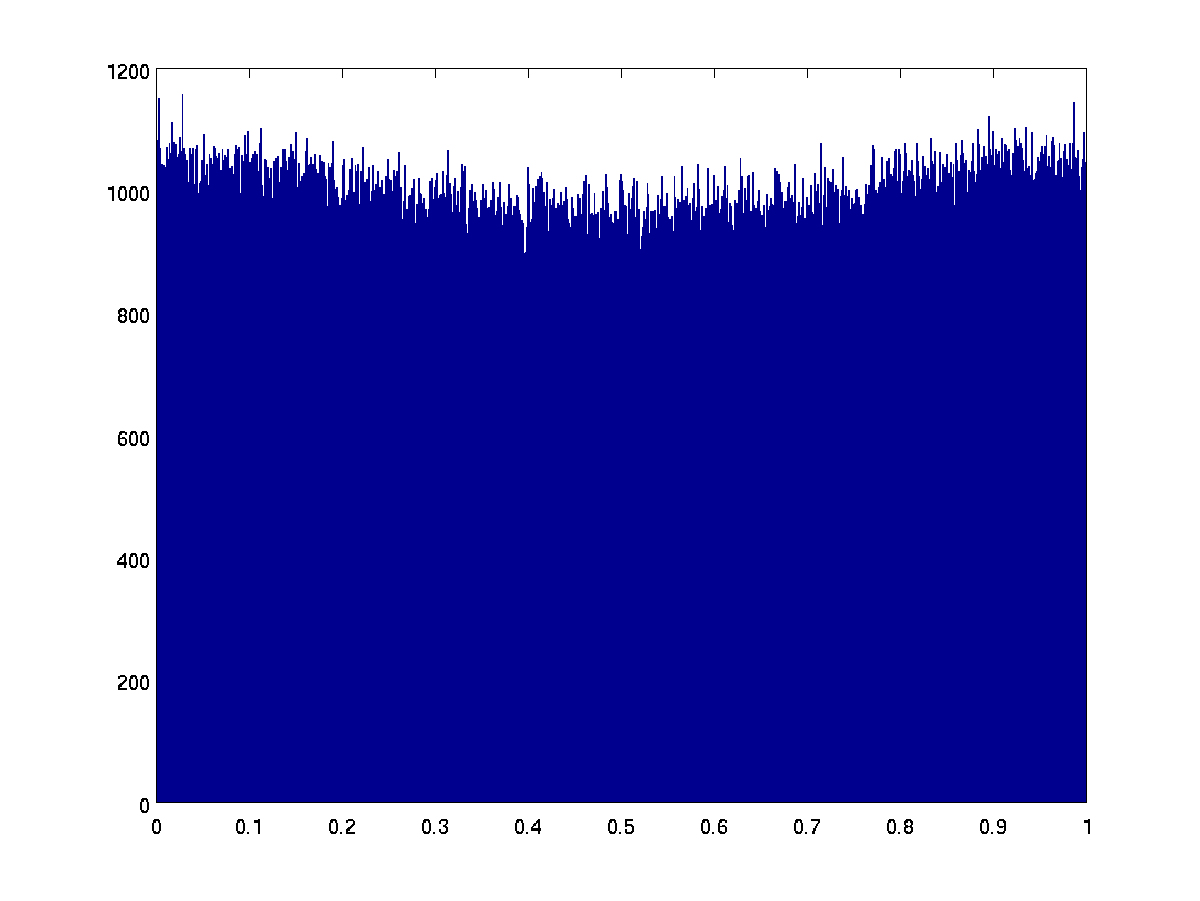
\includegraphics[scale=0.3]{qn_2_a_hist_2}
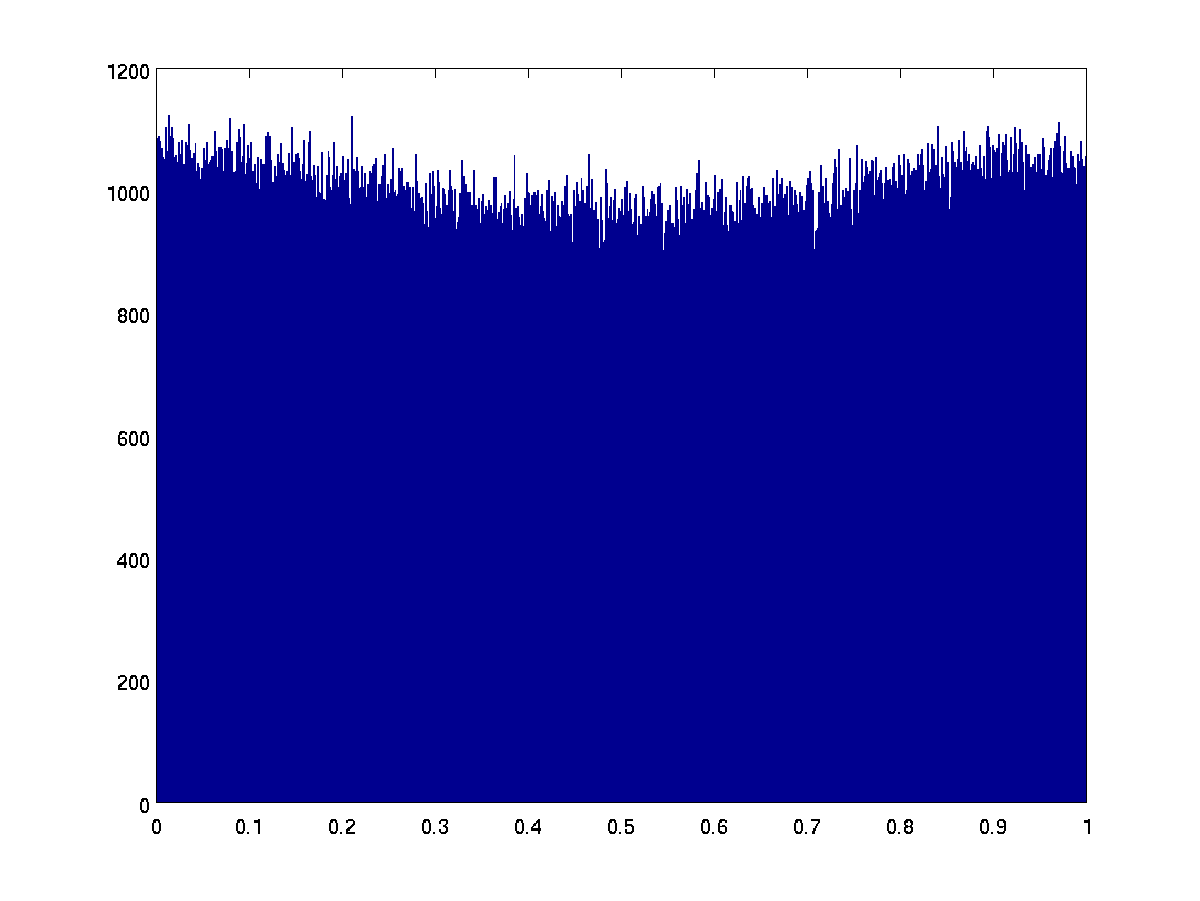
\includegraphics[scale=0.3]{qn_2_a_hist_3}
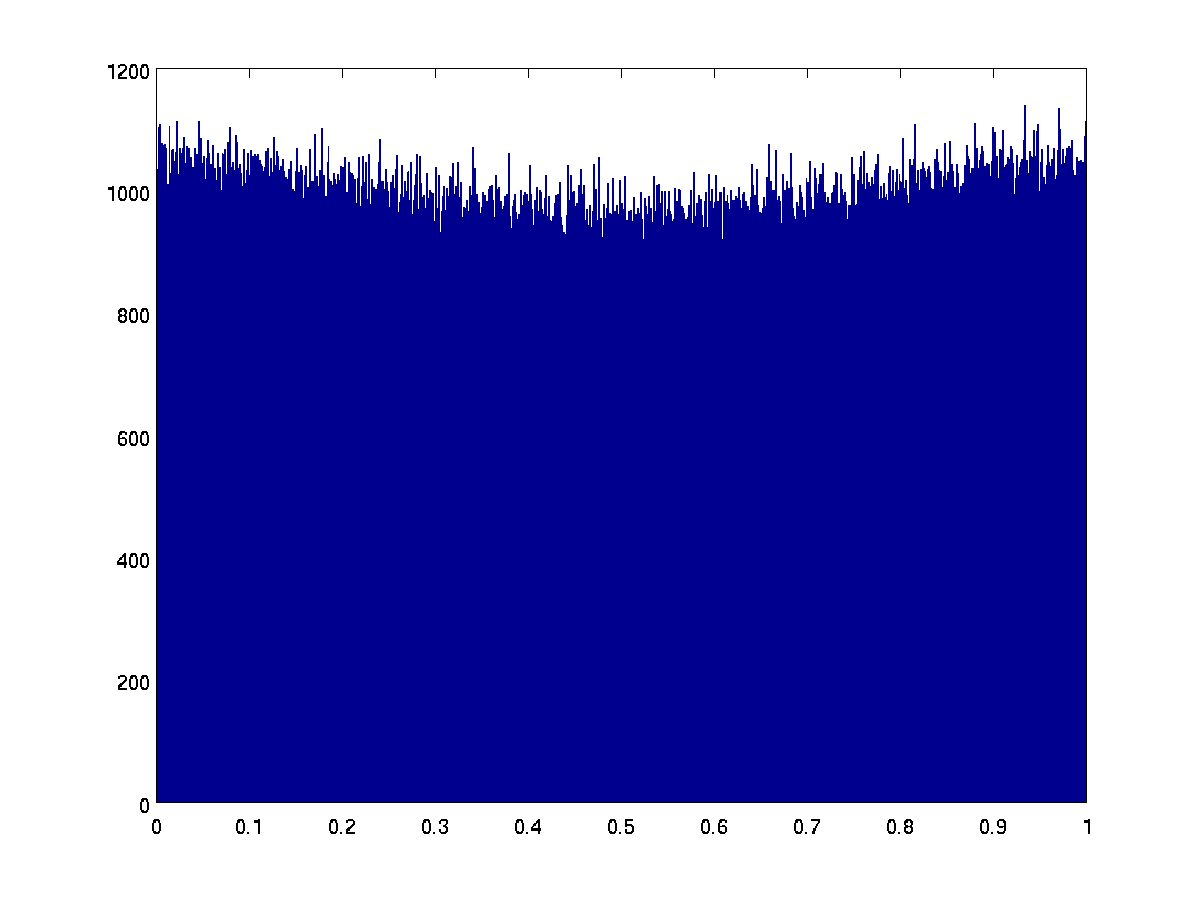
\includegraphics[scale=0.3]{qn_2_a_hist_4}
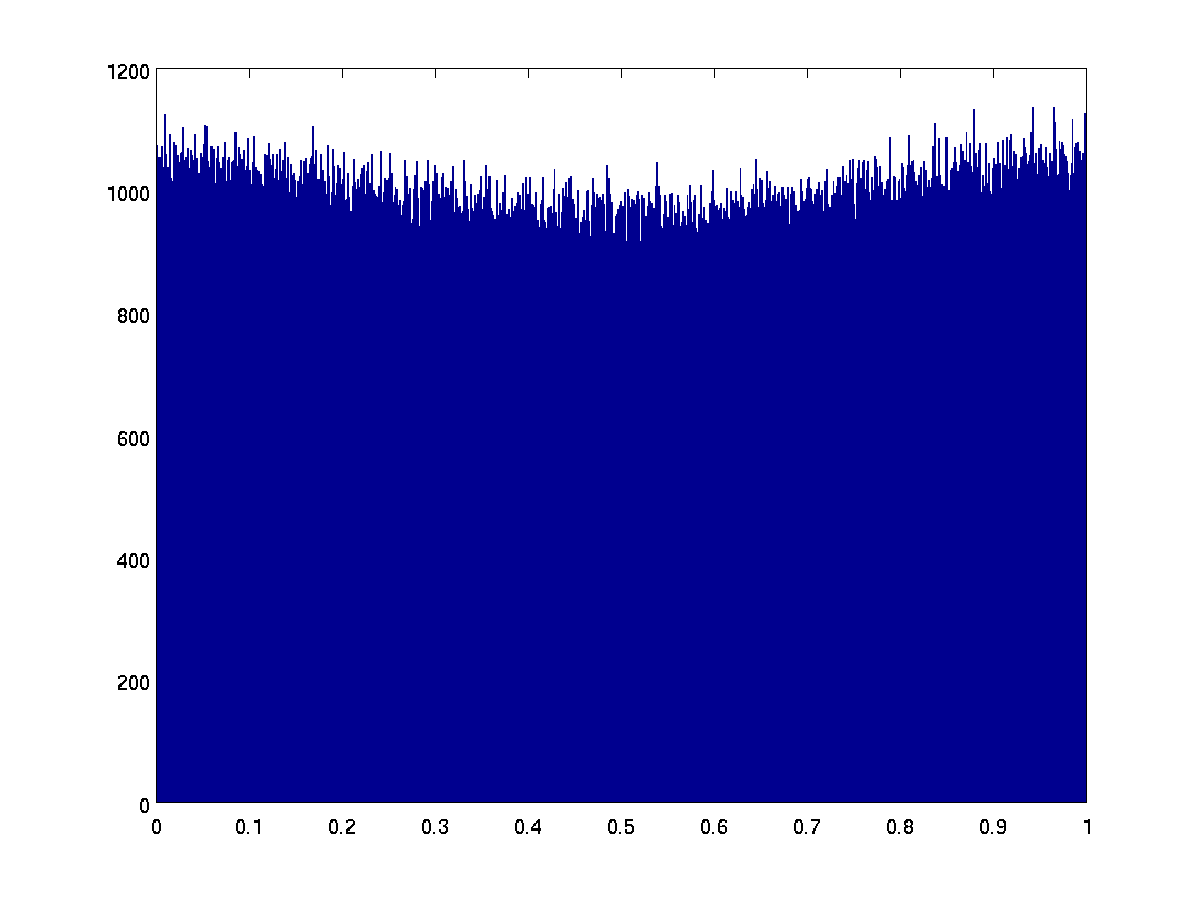
\includegraphics[scale=0.3]{qn_2_a_hist_5}
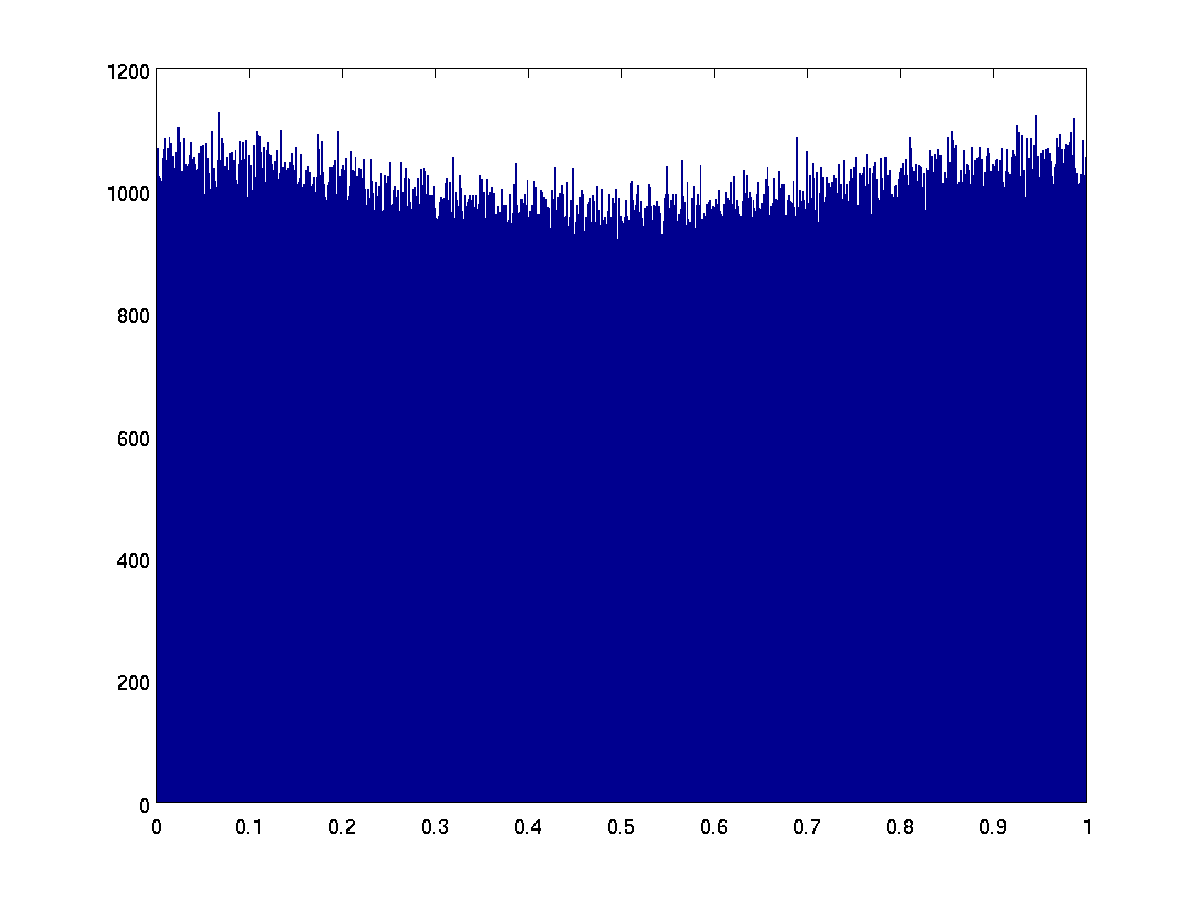
\includegraphics[scale=0.3]{qn_2_a_hist_6}
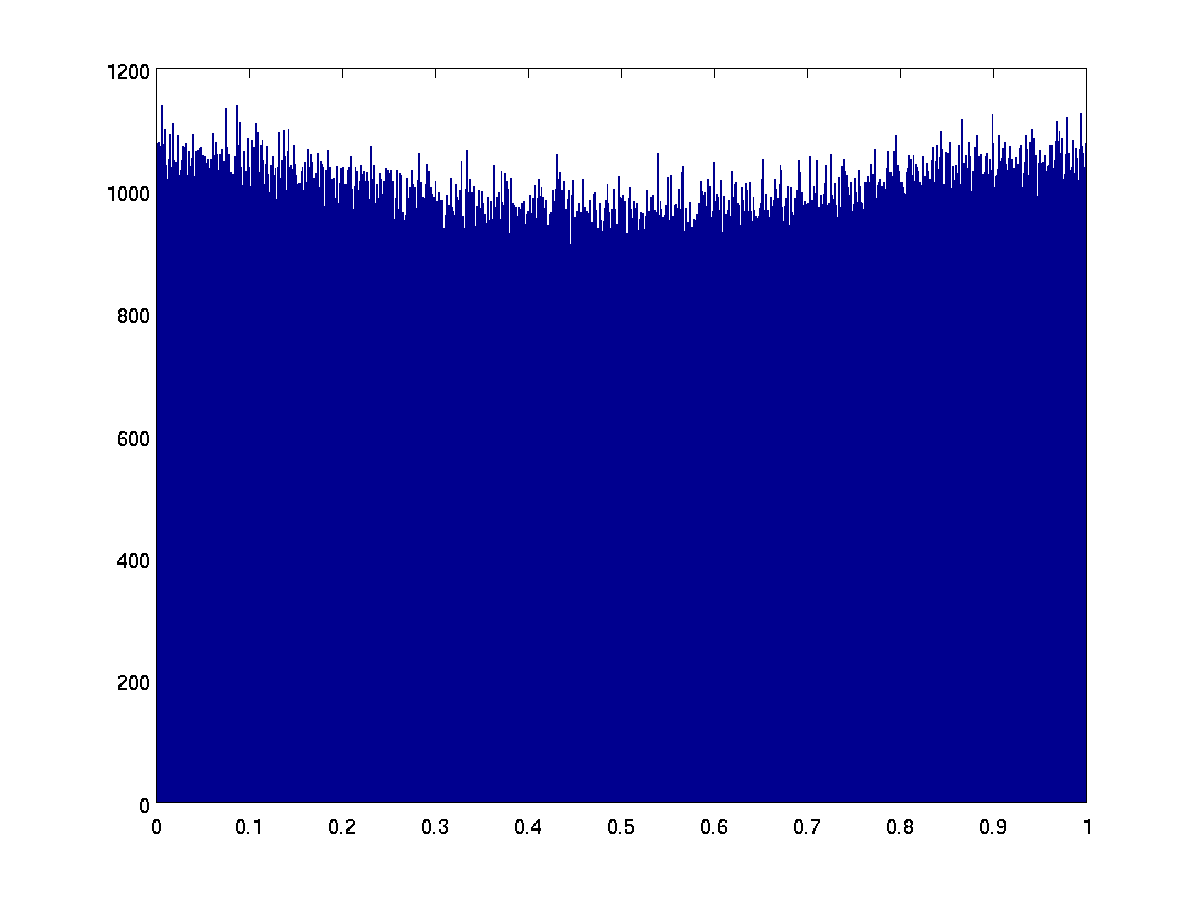
\includegraphics[scale=0.3]{qn_2_a_hist_7}
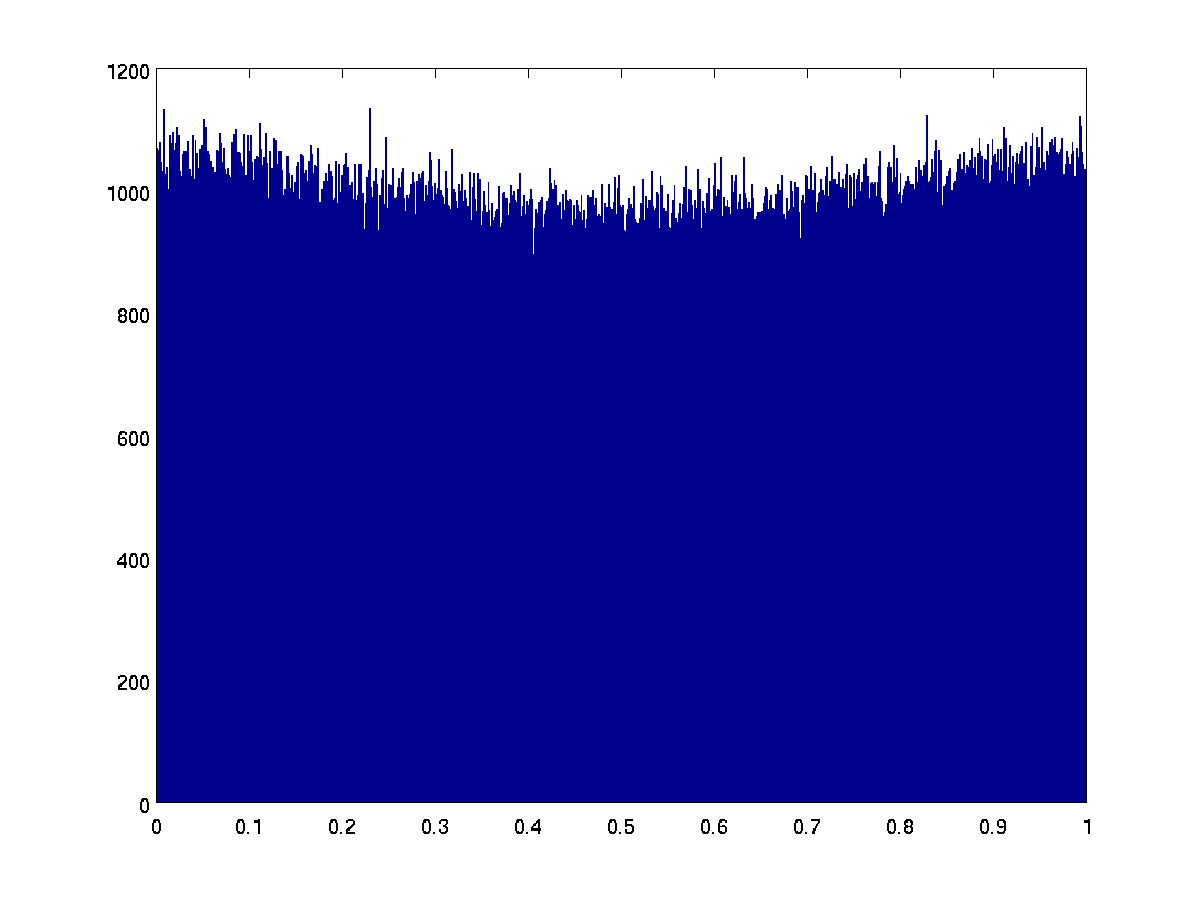
\includegraphics[scale=0.3]{qn_2_a_hist_8}
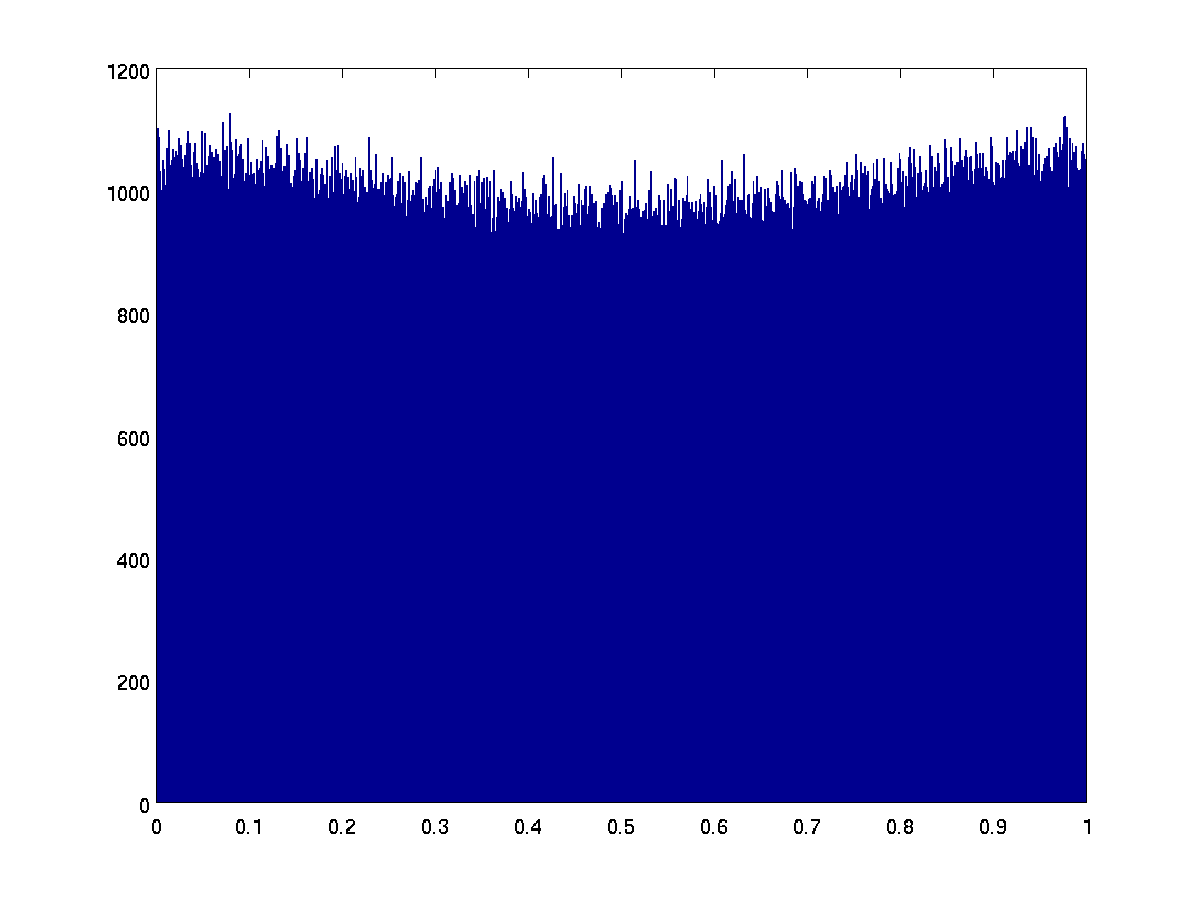
\includegraphics[scale=0.3]{qn_2_a_hist_9}
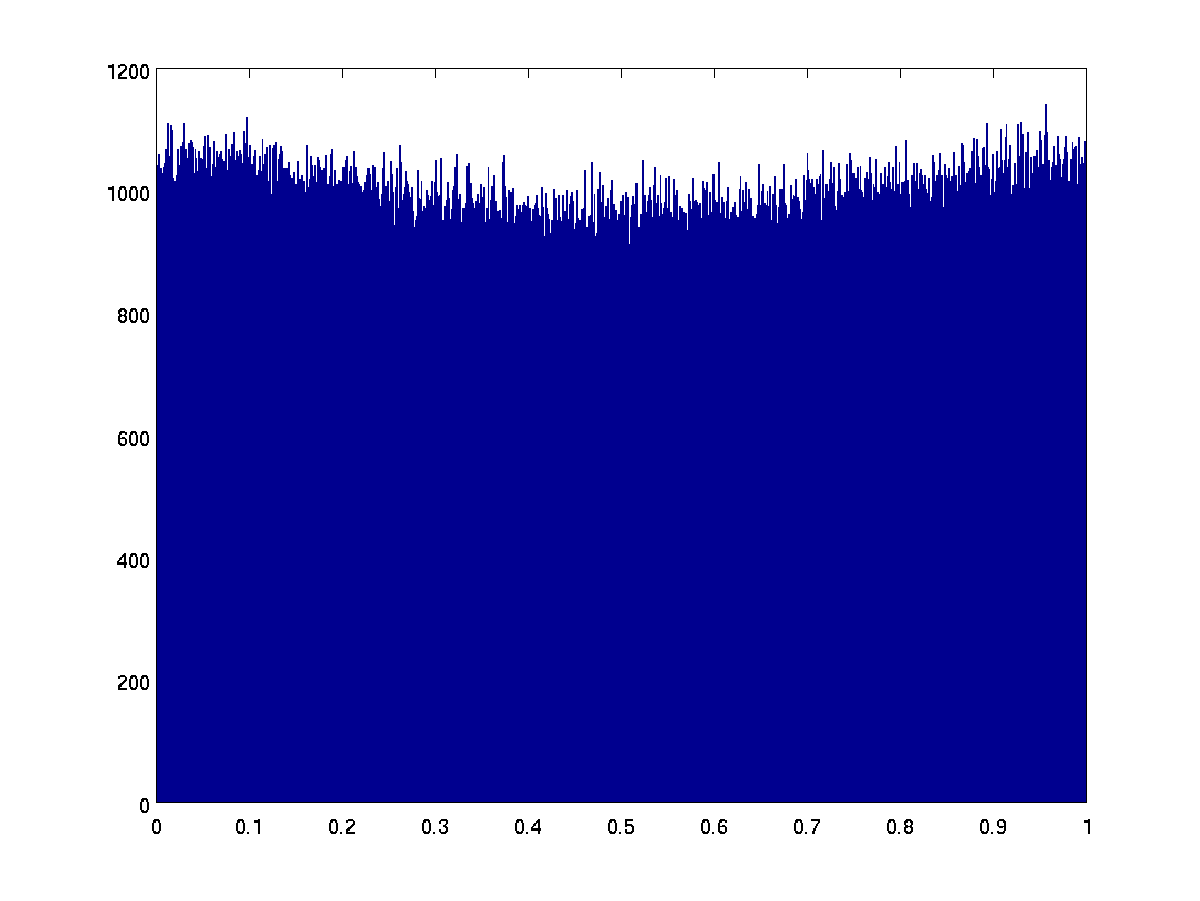
\includegraphics[scale=0.3]{qn_2_a_hist_10}

What these historgrams show is that TODO

\subsection{}
This code is available in \emph{Question\_2\_b\_c\_d.m} available at \url{https://github.com/adamjoshuagray/Honours_Ergodic_Theory/tree/master/Assignment_3}.

\subsection{}
Show TODO

Note that numerical verification is done in  \emph{Question\_2\_b\_c\_d.m} available at \url{https://github.com/adamjoshuagray/Honours_Ergodic_Theory/tree/master/Assignment_3}.

\subsection{}
The following is a plot of all the left eigenvalues of $ Q $ in the complex plane. 


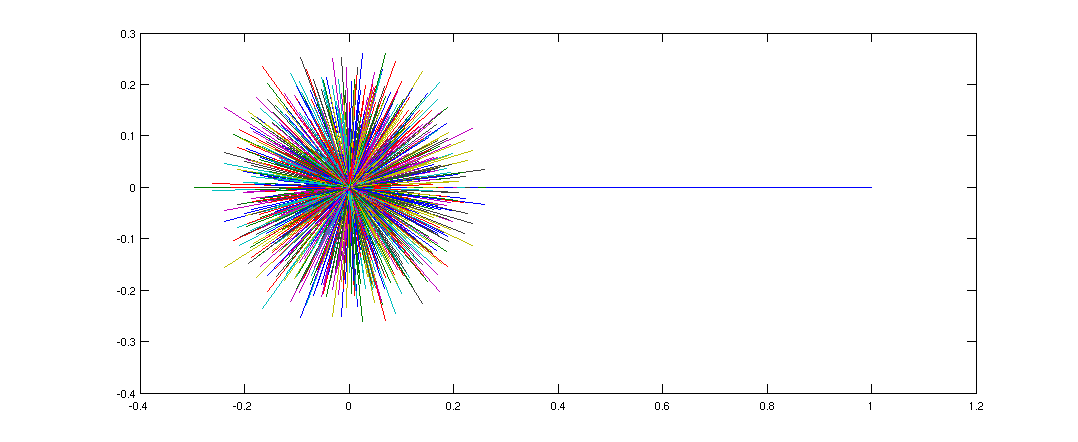
\includegraphics[scale=0.4]{qn_2_eigenvalues}


It is clear to see that there is only one eigenvalue equal to 1. We have also checked this in code in \emph{Question\_2\_b\_c\_d.m} available at \url{https://github.com/adamjoshuagray/Honours_Ergodic_Theory/tree/master/Assignment_3}.

The following is a plot of the left eigenvector corresponding to the eigenvalue 1.

\section{}
\subsection{}

Now note that $ S = h \circ T \circ h^{-1} $ or equivelently $ T = h^{-1} \circ S \circ h $.

As $ h $ and $ T $ are non-singular, so is $ S $ and thus by the composition of Perron-Frobenius operators
we can write
\begin{align}
    \mathcal{P}_T f = \left( \mathcal{P}_{h^{-1}} \circ \mathcal{P}_{S} \circ \mathcal{P}_{h} \right) f
\end{align}
or equivelently
\begin{align}
    \left( \mathcal{P}_{h} \circ \mathcal{P}_T \right) f = \left( \mathcal{P}_{S} \circ \mathcal{P}_{h} \right) f..
\end{align}
Now as $ \mathcal{P}_h f = g $ and by assumption $ \mathcal{P}_T f = f $ then
\begin{align}
    \mathcal{P}_h f = \mathcal{P}_s g
\end{align}
but we have also shown that $ \mathcal{P}_h f = g $
and so the result follows.
\subsection{}
From the lectures we know that $ \mathcal{P}_S g = g $ implies that $ g $ is an $ S $ invariant density, so the result is immediate.
A formal statement of that theorem along with it's proof is as follows
\begin{theorem}
\end{theorem}
\begin{proof}
  Suppose $ \mathcal{P}_{S} g = g $. Then we can say
  \begin{align}
    \int_A \mathcal{P}_S g d\mu = \int_A g d\mu.
  \end{align}
  Further we can say from the definition of the Perron-Frobenius operator that
  \begin{align}
    \int_A \mathcal{P}_{S} f d\mu = \int_{S^{-1}A} g d\mu
  \end{align}
  and so
  \begin{align}
    \int_A f d\mu = \int_{S^{-1}A} f d\mu
  \end{align}
  that is $ g $ is the density of a $ S $ invariant measure defined by
  \begin{align}
    \nu(A) = \int_{A} g d\mu.
  \end{align}
\end{proof}
\subsection{}
We wish to show that 
\begin{align}
  \int_I \log|T'(x)|d\mu_f(x) = \int_I \log|S'(x)|d\mu_g(x).
\end{align}
Starting from the definition of $ S $ we can write
\begin{align}
  \int_I \log|S'(x)|d\mu_g(x) &= \int_I \log|\left( h \circ T \circ h^{-1}(x) \right)'(x)|d\mu_g(x) \\
    &= \int_I \log|\left( h \circ T \circ h^{-1}(x) \right)'(x)|g(x)d\mu(x)
\end{align}
but then using the definition of $ g $ we can further write
\begin{align}
  \int_I \log|\left( h \circ T \circ h^{-1}(x) \right)'(x)|g(x)d\mu(x) &= \int_I \log|\left( h \circ T \circ h^{-1}(x) \right)'(x)|(f\circ h^{-1})(x) |h^{-1}(x)'|d\mu(x) \\
  &= 
\end{align}
Now let $ y = h^{-1}(x) $ so that $ d\mu(y) = h^{-1}(x)' d\mu(x) $ so we have
\begin{align}
  \int_{I} \log| \left( h'(T(y))\cdot T'(y) \cdot h \right)'(x) |
\end{align}

\section{}
\subsection{}
For $ T : I \lra I $ defined as
\begin{align}
  T(x) := 
  \begin{cases}
    2x  & 0 \leq x \leq \frac{1}{2} \\
    2(1-x) & \frac{1}{2} < x \leq 1
  \end{cases}
\end{align}
we have the following plot:


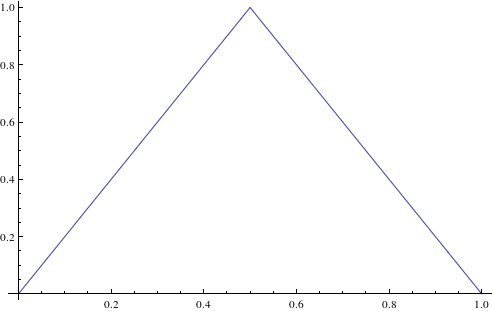
\includegraphics[scale=0.5]{qn_4_plot}

The T invariant density may be found in much the same way as for question 1.
If we let $ I_1 = \left[0,\frac{1}{2}\right] $ and $ I_2 = \left[ \frac{1}{2}, 1 \right] $ and choose the basis
  $\left\{ \mathds{1}_{I_1}, \mathds{1}_{I_2} \right\} $ then the associated matrix representation of the Perron-Frobenius operator is 
\begin{align}
  \left[ \begin{array}{cc} \frac{1}{2} & \frac{1}{2} \\ \frac{1}{2} & \frac{1}{2} \end{array} \right]
\end{align}
which has eigenvector $ (1,1) $ associated with eigenvalue $ 1 $ and so the $ T $ invariant density is $ \mathds{1}_{[0,1]} $, in other words the density is the uniform density (1).

\subsection{}
We have to do is show that 
\begin{align}
  g = (f \circ h^{-1})|\left( h^{-1} \right)'|
\end{align}
where $ f $ is the density of the ACIM associated with $ T $.

Now since $ f $ is the uniform density all we have to show is that
\begin{align}
 |\left( h^{-1} \right)'| = \frac{1}{\pi\sqrt{x(1-x)}}.
\end{align}
Now since $ h(x) = \sin^2(\frac{\pi x}{2}) $ we have that $ h^{-1}(x) = \frac{2}{\pi} \sin^{-1}(\sqrt{x}) $ and by differentiating we see that
\begin{align}
  \left( h^{-1}(x) \right)' = \frac{1}{\pi\sqrt{x(1-x)}}
\end{align}
and note that for $ x \in [0,1] $ this is positive so 
\begin{align}
| (h^{-1}(x))' | = \frac{1}{\pi\sqrt{x(1-x)}}
\end{align}
The last thing we have to show is that $ S(x) = \left( h \circ T \circ h^{-1} \right)(x) $ or equivelently $ T(x) = \left(h^{-1} \circ S \circ h \right)(x) $.

See that
\begin{align}
  T(x) &= \frac{2}{\pi} \sin^{-1}\left( \sqrt{4\sin^2\left(\frac{\pi  x}{2}\right)\left(1-\sin^2\left(\frac{\pi  x}{2}\right)\right) } \right) \\
    &= \frac{2}{\pi} \sin^{-1}\left( \sqrt{4\sin^2\left(\frac{\pi  x}{2}\right)\cos^2\left(\frac{\pi  x}{2}\right) } \right) \\
    &= \frac{2}{\pi} \sin^{-1}\left( 2 \sin\left(\frac{\pi  x}{2}\right)\cos\left(\frac{\pi  x}{2}\right) \right) \\
    &= \frac{2}{\pi} \sin^{-1}\left(  \sin\left(\pi  x\right)\right) \\
    &= \begin{cases} 2x & 0 \leq x \leq \frac{1}{2} \\ 2(1-x)  & \frac{1}{2} < x \leq 1 \end{cases}
\end{align}
and so this resolves the problem in that by using the result of Section 3.
That is, the density $ g $ is S-invariant.

\subsection{}
By using the result of question 3.3 we can calculate the  Lyapunov exponent of $ (I, \mathcal{B}, \mu_g, S) $ by just calculating the  Lyapunov exponent of $ (I, \mathcal{B}, \mu_f, T ) $. Since we have that $ f = 1 $ then we can just write
\begin{align}
  \int_{I} \log |T'(x)| d\mu_f(x) &= \int_{I} \log |T'(x)| d\mu \\
    &= \int_{0}^{1} \log 2 d\mu \\
    &= \log 2
\end{align}
\end{document}
